% ============================================================
%  中继无线传输系统设计 —— 组网设计方案
%  第 21 队
%  编译: xelatex design_proposal.tex
% ============================================================
\documentclass[12pt,a4paper]{ctexart}

% ---------- 页面设置 ----------
\usepackage[top=2.2cm,bottom=2.2cm,left=2.5cm,right=2.5cm,headheight=14pt]{geometry}
\usepackage{amsmath,amssymb}
\usepackage{graphicx}
\usepackage{float}
\usepackage{hyperref}
\usepackage{enumitem}
\usepackage{tabularx}
\usepackage{booktabs}
\usepackage{array}
\usepackage{multirow}
\usepackage{makecell}
\usepackage[table]{xcolor}
\usepackage{listings}
\usepackage{caption}
\usepackage{fancyhdr}
\usepackage{tikz}
\usetikzlibrary{arrows.meta,shapes,positioning,fit,backgrounds}

% ---------- 页面：允许底部不对齐，减少空白拉伸 ----------
\raggedbottom

% ---------- 段落首行缩进两字符 ----------
\setlength{\parindent}{2em}

% ---------- 表格样式 ----------
\renewcommand{\arraystretch}{1.25}
\setlength{\tabcolsep}{6pt}
\definecolor{tblhead}{HTML}{1e293b}
\definecolor{tblrowA}{HTML}{f8fafc}
\definecolor{tblrowB}{HTML}{f1f5f9}
\newcommand{\tblheaderstyle}{\sffamily\small\color{white}}
\captionsetup{font={small,stretch=0.95},labelfont=bf,skip=4pt}

% ---------- 代码块样式 ----------
\definecolor{codebg}{HTML}{f1f5f9}
\definecolor{codeframe}{HTML}{cbd5e1}
\definecolor{codecomment}{HTML}{64748b}
\lstset{
    basicstyle=\small\ttfamily,
    backgroundcolor=\color{codebg},
    frame=single,
    framerule=0.5pt,
    rulecolor=\color{codeframe},
    xleftmargin=8pt,
    xrightmargin=8pt,
    aboveskip=6pt,
    belowskip=6pt,
    breaklines=true,
    breakatwhitespace=false,
    columns=flexible,
    keepspaces=true,
    lineskip=2pt,
    commentstyle=\color{codecomment}\itshape,
    tabsize=2,
}

% ---------- 页眉页脚 ----------
\pagestyle{fancy}
\fancyhf{}
\fancyhead[L]{\small 中继无线传输系统设计}
\fancyhead[R]{\small 第 21 队}
\fancyfoot[C]{\thepage}
\renewcommand{\headrulewidth}{0.5pt}

% ---------- 列表间距：仅保留 enumerate 的紧凑样式 ----------
\setlist{nosep,leftmargin=*,itemsep=2pt,topsep=3pt,partopsep=0pt}

% ---------- 段落间距 ----------
\setlength{\parskip}{4pt plus1pt minus1pt}

% ---------- 超链接 ----------
\hypersetup{
    colorlinks=true,
    linkcolor=blue,
    urlcolor=cyan,
    citecolor=blue
}

\title{
    \vspace{1.5cm}
    {\Huge \textbf{中继无线传输系统设计}}\\[0.4cm]
    {\LARGE 组网设计方案}\\[0.8cm]
    \vspace{0.8cm}
}
\author{
    \textbf{第 21 队}\\[0.2cm]
    黄鹏峻 \quad 吴汉鹏 \quad 林金鑫 \quad 贾笛
}
\date{\today}

\begin{document}

\maketitle
\thispagestyle{empty}
\newpage

\tableofcontents
\newpage

% ============================================================
\section{项目概述}
% ============================================================

\subsection{项目背景与目标}

本项目面向无线自组织网络的设计与实现，以 Arduino Uno 为硬件平台、LoRa SX1278 为射频前端，构建一套支持多跳中继的无线传输系统。系统采用轻量级按需距离矢量路由协议（AODV-Lite），在 530\,MHz 频段上实现主节点、中继节点、终端节点的三层拓扑结构，并通过 USB 串口将网络状态实时桥接至 PC 端可视化界面。

从课程教学的角度审视，本设计全面对照了教学大纲的各项要求，涵盖基本指标与提高指标两个层面。具体的对应关系如表~\ref{tab:requirements} 所示。

\begin{table}[htbp]
\centering
\caption{课程要求与设计方案对应关系}
\label{tab:requirements}
\rowcolors{2}{tblrowA}{tblrowB}
\begin{tabularx}{\textwidth}{p{4.8cm}X}
\toprule
\rowcolor{tblhead}\tblheaderstyle 课程要求 & \tblheaderstyle 设计方案对应内容 \\
\midrule
完成 3 个无线设备的中继传输组网设计 &
4 节点（1 主节点 + 2 中继 + 1 终端）+ PC，支持多级中继 \\

白名单制度的设备入网过程 &
基于 JOIN/JOIN\_OK/JOIN\_NO 的三次握手入网，白名单决策由主节点执行 \\

主节点—中继节点—终端节点结构 &
明确三层角色分工，见第~\ref{sec:arch} 节系统架构 \\

传输拓扑信息维护，反映各节点变化 &
前端 ECharts 拓扑图实时渲染，Python StatsTracker 维护全量节点状态，20s 超时垃圾回收 \\

以帧结构形式传递三种以上信息 &
统一 16 字节帧结构，支持 RREQ/RREP/DATA/ACK/HB/JOIN/CMD 共 7 种消息类型 \\

结构化程序设计并绘制设计图 &
状态机驱动（sender）、窗口裁决（mainTerm）、非阻塞队列（relay），各节点均附完整流程图 \\

PC 端可视化控制，信道可读可设置可显示 &
FastAPI + WebSocket + ECharts 实时监控面板，信道配置面板支持频率/SF/功率下发 \\

动态新加入节点，4 节点 2 级中继 &
JOIN 协议支持任意时刻入网，RREQ 印章支持双跳路径（0x30$\to$0x21$\to$0x22$\to$0x10） \\

灵活可靠组网，拓扑结构维护 &
AODV-Lite 每轮重新探测 + 瓶颈 RSSI 选路 + 20s 超时拓扑清理 \\

组网设计方案（入网、维护、告警、在线调整） &
白名单入网流程、心跳保活、超时告警、信道参数在线下发、状态转移图 \\
\bottomrule
\end{tabularx}
\end{table}

\subsection{开发环境与工具链}

硬件方面，系统至少需要 3 套 Arduino Uno R3 开发板和同等数量的 LoRa SX1278 射频模块，当然也可以扩展到更多节点以适应更复杂的拓扑场景。微控制器固件使用 C/C++ 语言在 Arduino IDE 中编写，通过 SPI 接口驱动 LoRa 库实现无线收发。

PC 端由两部分组成：后端采用 Python 3.12 配合 FastAPI 框架、PySerial 串口库和 WebSocket 协议搭建；前端则是一个单页面应用，使用原生 HTML 和 JavaScript，界面样式借助 Tailwind CSS 实现快速布局，数据可视化部分依赖 ECharts 5.5 图表库。

通信参数方面，系统默认工作在 530\,MHz 频段，扩频因子取值范围为 SF7 至 SF12，发射功率可在 2 至 20\,dBm 之间调节。出厂默认配置为 SF7、17\,dBm，这是兼顾通信速率与覆盖距离的折中选择。

% ============================================================
\section{系统架构}
\label{sec:arch}
% ============================================================

\subsection{网络拓扑结构}

系统由四类节点构成三级网络拓扑，各节点的角色和职责明确区分。

第一类是 PC 网关，它运行 Python 后端服务，通过 USB 串口与主节点物理相连，同时充当 Web 服务器为浏览器提供可视化界面。需要指出的是，PC 网关并不直接参与无线通信，它的作用更像是一个"翻译官"——将空中无形的 LoRa 信号转换为人类可以直观理解的图表和日志。

第二类是主节点 mainTerm，其节点 ID 固定为 \texttt{0x10}。它在 LoRa 网络中扮演目的节点的角色，承担着三重核心任务：RREQ 路由收集与瓶颈 RSSI 裁决、串口桥接 PC、以及入网白名单决策。硬件为 Arduino Uno 搭配 LoRa SX1278 模块。

第三类是中继节点 relayTerm，节点 ID 可配置为 \texttt{0x21}、\texttt{0x22} 等。中继节点的核心使命是对途经的 RREQ 帧进行 RSSI 盖章并广播转发，同时在 RREP/DATA/ACK 阶段实现选择性透明转发。其设计精髓在于非阻塞队列管理和 ID 差异化退避机制，这两个设计点将在第~\ref{sec:nodes} 节详细展开。烧录固件时需修改 \texttt{MY\_NODE\_ID} 宏以区分不同中继。

第四类是终端节点 sender，节点 ID 固定为 \texttt{0x30}。它是整个通信过程的总发起者——决定何时探测路由、何时发送数据、何时等待确认。其行为完全由一套有限状态机（FSM）驱动，在 IDLE、WAITING\_RREP、WAITING\_ACK 三个状态之间有序切换。

\subsection{数据流架构}

系统的完整数据流链路可以归纳为三段。无线段：sender 经过零跳、一跳或两跳中继最终到达 mainTerm，所有无线传输均使用 530\,MHz LoRa，SF7 扩频因子。有线段：mainTerm 将收到的无线帧以原始二进制形式通过 USB 串口（9600 baud）发送给 Python 后端，后者解析为结构化 JSON 后经 WebSocket 推送给浏览器。控制反向：用户在浏览器上的操作（如打开串口、下发信道配置）沿 WebSocket $\to$ Python $\to$ Serial $\to$ mainTerm $\to$ LoRa 的反向路径抵达目标节点。

\begin{figure}[htbp]
\centering
\includegraphics[width=\textwidth]{fig_system_architecture.jpg}
\caption{系统整体架构}
\label{fig:sysarch}
\end{figure}

图~\ref{fig:sysarch} 从全局视角呈现了上述四类节点的物理部署关系和信号流向：左侧为无线 LoRa 多跳网络，右侧为 PC 端的数据处理与可视化链路，中间以 USB 串口为纽带将两个世界桥接起来。

% ============================================================
\section{通信协议设计}
\label{sec:protocol}
% ============================================================

\subsection{统一帧结构}

在无线多跳网络中，如果每种消息都采用不同的帧格式，不仅会增加接收端的解析复杂度，更容易引入难以排查的边界 bug。基于这一考量，本系统设计了统一的 16 字节定长帧结构——所有消息类型共用同一格式模板，仅通过 \texttt{msgType} 字段区分语义，而 \texttt{data[8]} 字段则在不同的消息类型中承载截然不同的含义。帧结构的完整定义见表~\ref{tab:framestruct}。

\begin{table}[htbp]
\centering
\caption{统一帧结构定义（16 字节）}
\label{tab:framestruct}
\rowcolors{2}{tblrowA}{tblrowB}
\begin{tabularx}{\textwidth}{c l c c >{\raggedright\arraybackslash}X}
\toprule
\rowcolor{tblhead}\tblheaderstyle 偏移 & \tblheaderstyle 字段 & \tblheaderstyle 长度 & \tblheaderstyle 类型 & \tblheaderstyle 说明 \\
\midrule
0  & \texttt{head[0]} & 1B & uint8 & 魔术字高字节，固定 \texttt{0x4C}（'L'） \\
1  & \texttt{head[1]} & 1B & uint8 & 魔术字低字节，固定 \texttt{0x6F}（'o'） \\
2  & \texttt{srcId}   & 1B & uint8 & 原始发送者节点 ID \\
3  & \texttt{destId}  & 1B & uint8 & 最终目标节点 ID \\
4  & \texttt{msgType} & 1B & uint8 & 消息类型（见第~\ref{sec:msgtypes} 节） \\
5  & \texttt{pathId}  & 1B & uint8 & 路由发现序号，每轮递增 \\
6  & \texttt{count}   & 1B & uint8 & 语义随 msgType 变化（见第~\ref{tab:countdata} 页） \\
7--14 & \texttt{data[8]} & 8B & uint8[8] & 语义随 msgType 变化（见第~\ref{tab:countdata} 页） \\
15 & \texttt{checksum}& 1B & uint8 & 异或校验和，覆盖偏移 2--14 共 13 字节 \\
\bottomrule
\end{tabularx}
\end{table}

\begin{figure}[htbp]
\centering
\includegraphics[width=\textwidth]{fig_frame_structure.jpg}
\caption{统一帧结构可视化（16 字节）}
\label{fig:framestruct}
\end{figure}

图~\ref{fig:framestruct} 以内存布局图的形式直观展示了 16 字节帧的字段划分与偏移量。其中校验和覆盖 \texttt{srcId} 至 \texttt{data[7]} 共计 13 字节，帧头 \texttt{head[0..1]} 和校验和自身不参与异或运算——这样做的理由很简单：帧头是固定常量，校验和是计算结果，将它们纳入校验范围并无意义。

\texttt{count} 字段和 \texttt{data[8]} 字段的语义随着 \texttt{msgType} 的不同会发生根本性的变化，这是统一帧设计中最需要读者注意的地方。例如，当 \texttt{msgType = 0x10}（RREQ）时，\texttt{count} 表示已收集的 RSSI 印章对数，\texttt{data[]} 中按 $\{id, rssi\}$ 逐对排列；而当 \texttt{msgType = 0x11}（RREP）时，\texttt{count} 表示选中的中继 ID 数量，\texttt{data[]} 中直接排列中继 ID。详细的语义映射见表~\ref{tab:countdata}。

\begin{table}[htbp]
\centering
\caption{count 与 data[8] 的语义映射}
\label{tab:countdata}
\rowcolors{2}{tblrowA}{tblrowB}
\begin{tabularx}{\textwidth}{l l >{\raggedright\arraybackslash}p{5.8cm} >{\raggedright\arraybackslash}X}
\toprule
\rowcolor{tblhead}\tblheaderstyle msgType & \tblheaderstyle count 含义 & \tblheaderstyle data[0..7] 内容 & \tblheaderstyle data[7] 特殊用途 \\
\midrule
RREQ (0x10) & 印章对数 ($\le$4) &
$\{id_1,\ rssi_1,\ \ldots,\ id_n,\ rssi_n\}$ 逐对排列 &
当 count $<$ 4 时，嵌入末跳 RSSI (int8) \\

RREP (0x11) & 中继 ID 数 ($\le$2) &
中继 ID 列表（每 ID 占 1 字节） &
无；mainTerm 生成时 data[7] = 0x00 \\

DATA (0x01) & 中继 ID 数 ($\le$2) &
中继 ID 列表 + 载荷（sampleCounter、0xAB） &
当 count $<$ 4 时，嵌入末跳 RSSI (int8) \\

ACK  (0x02) & 中继 ID 数 ($\le$2) &
中继 ID 列表（每 ID 占 1 字节） &
无；mainTerm 生成时 data[7] = 0x00 \\

JOIN (0x20) & 0 &
data[0] = 角色码（1=中继，2=终端） &
-- \\

JOIN\_OK (0x21) & 0 &
data[0..1] = \texttt{0xAC 0x00} &
-- \\

JOIN\_NO (0x22) & 0 &
data[0] = 拒绝原因码 &
-- \\

CMD  (0x04) & 0 &
ASCII 命令字符串 &
-- \\
\bottomrule
\end{tabularx}
\end{table}

\subsection{校验和算法}

校验和采用逐字节异或运算，用 C 语言的视角来看就是一句话的事：

\begin{lstlisting}[]
checksum = srcId ^ destId ^ msgType ^ pathId ^ count
         ^ data[0] ^ data[1] ^ data[2] ^ data[3]
         ^ data[4] ^ data[5] ^ data[6] ^ data[7]
\end{lstlisting}

之所以选择异或而非求和取模，是因为异或运算在 Arduino 的 ATmega328P 上只需单条指令即可完成，不涉及进位处理，对 16\,MHz 主频的微控制器而言几乎不占 CPU 时间。校验覆盖范围排除了帧头（固定常量，无校验价值）和校验和自身（循环依赖），仅针对有效载荷的 13 字节进行完整性保护。

\subsection{消息类型定义}
\label{sec:msgtypes}

系统共定义了七种消息类型，覆盖了路由探测、数据传输、确认应答、入网管理和信道配置四大功能域，见表~\ref{tab:msgtypes}。这一数量远超课程要求的"三种以上"，为系统在不同工作阶段提供了精确的语义表达手段。

\begin{table}[htbp]
\centering
\caption{消息类型常量定义}
\label{tab:msgtypes}
\rowcolors{2}{tblrowA}{tblrowB}
\begin{tabularx}{\textwidth}{l c c l >{\raggedright\arraybackslash}X}
\toprule
\rowcolor{tblhead}\tblheaderstyle 常量名 & \tblheaderstyle 值 & \tblheaderstyle 方向 & \tblheaderstyle 名称 & \tblheaderstyle 说明 \\
\midrule
MSG\_RREQ    & 0x10 & sender $\to$ 广播       & 路由发现请求   & 终端发起路径探测，中继逐跳 RSSI 盖章 \\
MSG\_RREP    & 0x11 & mainTerm $\to$ sender   & 路由发现应答   & 主节点沿选中路径回传裁决结果 \\
MSG\_DATA    & 0x01 & sender $\to$ mainTerm   & 用户数据传输   & 沿选中路径发送采样数据 \\
MSG\_ACK     & 0x02 & mainTerm $\to$ sender   & 数据确认应答   & 确认数据已成功接收，发 3 份 \\
MSG\_HB      & 0x03 & 各节点 $\to$ mainTerm   & 心跳保活       & 周期性发送，维持拓扑活跃状态 \\
MSG\_CMD     & 0x04 & PC $\to$ 目标节点       & 下行命令       & PC 通过主节点向任意节点下发信道配置 \\
MSG\_CMD\_ACK& 0x05 & 目标节点 $\to$ PC       & 命令应答       & 确认命令已执行 \\
MSG\_JOIN    & 0x20 & 新节点 $\to$ mainTerm   & 入网请求       & 节点上电后向主节点发起入网 \\
MSG\_JOIN\_OK& 0x21 & mainTerm $\to$ 新节点   & 入网允许       & 主节点白名单校验通过 \\
MSG\_JOIN\_NO& 0x22 & mainTerm $\to$ 新节点   & 入网拒绝       & 主节点白名单校验失败 \\
\bottomrule
\end{tabularx}
\end{table}

简要概括这七种消息的分工：RREQ 和 RREP 构成路由控制平面，负责在每次通信前找到一条信号质量可接受的路径；DATA 和 ACK 构成数据传输平面，负责将采样数据可靠地从终端送达主节点并取得确认；HB 维持拓扑心跳，使整网感知各节点的存活状态；JOIN 系列消息管控入网安全，确保只有白名单内的设备能够加入网络；CMD 系列则提供了一条从 PC 浏览器直达任意节点的带外管理通道。

% ============================================================
\section{各节点程序设计}
\label{sec:nodes}
% ============================================================

\subsection{终端节点 sender（0x30）}

\subsubsection{设计概述}

终端节点是通信过程的发起者和最终受益者——它决定何时探测路由、何时沿选定路径发送数据、以多大的耐心等待确认。如果用一个词概括 sender 的程序架构，那就是"状态机"。三个状态、四条转移路径、两个超时计时器，构成了 sender 全部的行为逻辑。

\subsubsection{状态机设计}

终端节点维护三个核心状态，其定义见表~\ref{tab:senderstates}。

\begin{table}[htbp]
\centering
\caption{sender 状态定义}
\label{tab:senderstates}
\rowcolors{2}{tblrowA}{tblrowB}
\begin{tabularx}{\textwidth}{c >{\raggedright\arraybackslash}X c}
\toprule
\rowcolor{tblhead}\tblheaderstyle 状态 & \tblheaderstyle 说明 & \tblheaderstyle 超时 \\
\midrule
IDLE &
空闲状态，等待 10s 间隔后检查路由有效性，若路由过期或无效则发起 RREQ &
-- \\

WAITING\_RREP &
RREQ 已发送，等待主节点回传 RREP &
2000\,ms \\

WAITING\_ACK &
DATA 已发送，等待主节点回传 ACK 确认 &
2000\,ms \\
\bottomrule
\end{tabularx}
\end{table}

\subsubsection{状态转移逻辑}

状态机的运转逻辑可以概括为四条转移路径。

第一条，IDLE $\to$ WAITING\_RREP。当路由缓存因首次启动、ACK 超时后被清除、或路由年龄超过 10\,s 而失效时，sender 广播 RREQ 帧并递增 \texttt{pathId}，随后进入等待状态。

第二条，IDLE $\to$ WAITING\_ACK。当路由缓存仍然有效时，sender 跳过探测环节，直接使用已缓存的中继路径发送 DATA 帧。

第三条，WAITING\_RREP $\to$ WAITING\_ACK。在超时前收到有效 RREP 时，解析选中的中继路径并存入路由缓存，紧接着发送 DATA。

第四条，WAITING\_ACK $\to$ IDLE。这是最关键的一步转移——收到 ACK 后，sender 强制清除路由缓存（确保下一轮重新探测，使路径选择始终反映当前电磁环境），然后启动 10\,s 的静默等待。若 2\,s 内未收到 ACK，则标记路由无效并回到 IDLE，等待下一周期重新尝试。

\begin{figure}[htbp]
\centering
\includegraphics[width=0.85\textwidth]{fig_sender_fsm.jpg}
\caption{sender 节点状态转移图（FSM）}
\label{fig:senderfsm}
\end{figure}

图~\ref{fig:senderfsm} 以图形化方式给出了上述三状态有限状态机的完整视图，状态间的转移条件和超时回退路径一目了然。

\subsubsection{关键数据结构}

sender 仅维护一个路由表项，这是因为在单目的节点的拓扑中，无需维护复杂的多条目路由表。\texttt{RouteEntry} 结构体封装了目标节点 ID、中继数量与 ID 列表、路由序号和时间戳，外加一个有效性标志位。

\begin{lstlisting}[]
struct RouteEntry {
    uint8_t  destId;        // 目标节点 ID (固定 0x10)
    uint8_t  relayCount;    // 中继数 (0=直达, 1~2=中继)
    uint8_t  relays[2];     // 中继 ID 列表
    uint8_t  pathId;        // 路由发现序号
    uint32_t timestamp;     // 路由建立时间
    bool     valid;         // 路由有效性标志
};
RouteEntry route;           // 唯一路由表项
\end{lstlisting}

\subsubsection{主循环伪代码}

\begin{lstlisting}[]
function loop():
    checkForPacket()           // 非阻塞收包检查
    now = millis()

    if discState == IDLE:
        if now - lastAction >= 10000:
            if route 无效或过期:
                sendRREQ()
                dataPending = true
            else:
                sendData()
                dataPending = false

    else if discState == WAITING_RREP:
        if now - rreqSendTime > 2000:
            discState = IDLE   // 超时回退

    else if discState == WAITING_ACK:
        if now - ackSendTime > 2000:
            discState = IDLE
            route.valid = false  // 路由失效
\end{lstlisting}

\subsection{中继节点 relayTerm（0x21 / 0x22）}

\subsubsection{设计概述}

中继节点是整个 AODV-Lite 协议最核心的执行者。它的任务看似简单——收到帧、盖章、转发——但要在多中继同时收到同一广播帧的场景下避免空中碰撞、防止环路转发、保证转发时机错开，就需要精巧的工程设计。本系统的中继方案建立在三个支柱之上：非阻塞转发队列、ID 差异化退避、以及基于四元组的转发去重保护。

\subsubsection{RREQ 处理流程}

中继节点收到一个无线帧之后，首先执行六级校验，任何一级未通过则丢弃该帧。

第一级，长度校验。LoRa 帧必须恰好为 16 字节，否则记录 \texttt{badSize} 并丢弃。

第二级，魔术字校验。帧头两个字节必须为 \texttt{0x4C 0x6F}，否则记录 \texttt{badMagic} 并丢弃。

第三级，地址过滤。若目标地址等于本节点 ID，说明该帧为发给自己的（如 RREP/DATA/ACK 沿路径回传的情况），但在 RREQ 阶段目标地址永远是 mainTerm 的 0x10，因此中继收到的 destId 为本节点的 RREQ 可直接丢弃。

第四级，校验和验证。对偏移 2 至 14 的 13 字节做逐字节异或，结果必须等于 \texttt{checksum} 字段。

第五级，防环检查。遍历 data[] 中已有的 RSSI 印章，若发现本节点 ID 已被盖章，则说明该 RREQ 曾经经过本节点并已被转发过，丢弃以阻断环路。

第六级，容量检查。若 \texttt{count >= 4}，印章区已满，无法继续盖章，丢弃。

通过全部校验后，中继执行 RSSI 盖章操作：在 \texttt{data[count*2]} 位置写入本节点 ID，\texttt{data[count*2+1]} 位置写入当前 LoRa 接收信号强度（int8 类型的有符号值），随后递增 \texttt{count} 并重新计算校验和。

盖章完成后并非立即发送，而是根据跳数和节点 ID 计算退避时间。单跳场景（count $\le$ 1）的退避公式为 $T = (\text{ID 末 4 位}) \times 80 + 10$\,ms；多跳场景（count $>$ 1）的退避公式为 $T = (\text{ID 末 4 位}) \times 40 + 100$\,ms。以 0x21 和 0x22 为例，单跳退避分别为 90\,ms 和 170\,ms，两者之间拉开 80\,ms 的安全间隙，天然避免了同时转发造成的空中碰撞。

最后一步是非阻塞入队：将盖章后的帧放入容量为 2 的 pending 队列，由主循环中的 \texttt{servicePending()} 函数异步完成实际发送。每帧仅发送 1 份——发送多个副本虽然理论上提高可靠性，但实际上会长时间占用信道，导致后续的中继无法收到下一跳的 RREQ，反而破坏了多跳链的连续性。

\begin{figure}[htbp]
\centering
\includegraphics[width=0.8\textwidth]{fig_relay_rreq_flow.jpg}
\caption{relayTerm RREQ 处理流程}
\label{fig:relayflow}
\end{figure}

图~\ref{fig:relayflow} 将上述六级校验链路及后续的盖章、退避、入队操作以流程图形式完整呈现。

\subsubsection{RREP / DATA / ACK 处理流程}

对于 RREP、DATA 和 ACK 三类帧，中继的处理逻辑相对简洁。首先解析帧的 \texttt{data[]} 字段提取中继 ID 列表，然后判断本节点是否在路径中——若不在，则丢弃（该路径未选中本节点）。若在路径中，则进一步检查四元组去重缓存：若该帧的 \texttt{(srcId, destId, pathId, msgType)} 组合已被转发过，则跳过；否则标记为已转发，然后通过 LoRa 透明转发。

转发策略因帧类型而异：RREP 和 DATA 仅发 1 份即可，因为它们沿已确定的路径传输，路径上的每个节点都会各司其职；ACK 在中继侧发 2 份——这比源头 mainTerm 的 3 份略少，是一种分级冗余策略，在确保可接受可靠性的同时降低了对信道的占用。

\subsubsection{非阻塞转发队列}

\begin{table}[htbp]
\centering
\caption{非阻塞转发队列参数}
\rowcolors{2}{tblrowA}{tblrowB}
\begin{tabularx}{\textwidth}{l c >{\raggedright\arraybackslash}X}
\toprule
\rowcolor{tblhead}\tblheaderstyle 参数 & \tblheaderstyle 值 & \tblheaderstyle 说明 \\
\midrule
MAX\_PENDING     & 2    & 最大同时待转发帧数，防止内存溢出 \\
副本数 (retries) & 1    & 每帧只发一次，减少信道占用 \\
发送间隔         & 30ms & 相邻 pending 帧间最小间隔 \\
\bottomrule
\end{tabularx}
\end{table}

\subsubsection{转发去重机制}

中继节点维护一个容量为 4 的环形缓存，每条记录存储已转发帧的四元组 \texttt{(srcId, destId, pathId, msgType)}。每次准备转发前先线性扫描该缓存，若匹配则说明该帧已被处理过，直接丢弃。这个简单的机制有效防止了同一帧在中继之间乒乓循环——在 LoRa 广播网络中，节点 B 可能先收到节点 A 的转发，再收到原始 sender 的广播，如果不做去重，B 会把同样的帧转发两次甚至更多次。

\subsubsection{主循环伪代码}

\begin{lstlisting}[]
function loop():
    handlePacket()       // 非阻塞收包 (每 5ms)
    servicePending()     // 非阻塞发送队列服务

function handlePacket():
    pkt = LoRa.parsePacket()
    if pkt.len != 16: return
    rx = 读取帧
    if rx.magic != 0x4C6F: 记录并返回
    if rx.destId == MY_ID: 记录并返回  // RREQ 目标永远是 0x10
    if !verifyChecksum(rx): 记录并返回

    switch rx.msgType:
        case RREQ: handleRREQ(rssi)
        case RREP: handleRREP()
        case DATA: handleDATA()
        case ACK:  handleACK()

function handleRREQ(rssi):
    if rx.count >= 4: return              // 印章满
    if 本节点已在 stamps 中: return         // 防环
    在 data[count*2] 写入 MY_ID, rssi
    rx.count++
    重算校验和
    计算退避
    enqueueForward(&rx, backoff, rssi)    // 非阻塞入队

function handleRREP/handleDATA/handleACK():
    if 本节点不在 relays 列表中: return
    if wasForwarded(四元组): return        // 去重
    markForwarded(四元组)
    LoRa 透明转发
\end{lstlisting}

\subsection{主节点 mainTerm（0x10）}

\subsubsection{设计概述}

主节点是系统中最忙碌的设备。一方面，它是 LoRa 网络中所有路由探测帧（RREQ）的最终目的地，承担着收集、比较和裁决多路径信号质量的核心职责；另一方面，它又是无线世界与 PC 世界之间的唯一桥梁——将空中收到的每一帧通过 USB 串口实时转发给 Python 后端。这种双重角色意味着 mainTerm 的程序设计必须在 LoRa 接收灵敏度与串口转发及时性之间取得平衡。

\subsubsection{RREQ 收集与裁决}

\paragraph{窗口机制}
每个新的 \texttt{pathId} 会触发一个持续 500\,ms 的收集窗口。在这半秒钟内，所有携带相同 \texttt{pathId} 的 RREQ——无论来自直达路径还是经过一个或两个中继——都被集中存入一个容量为 6 的候选数组中。窗口到期后，裁决逻辑启动。

\paragraph{去重合并策略}
LoRa 网络中同一帧可能被多次接收（比如 sender 广播被中继 A 收到后转发，又被中继 B 转发，mainTerm 可能先后收到 A 的版本和 B 的版本）。对于 \texttt{(pathId, srcId, stampCount, relay IDs)} 完全相同的重复帧，仅保留其中瓶颈 RSSI 最好的一份。而不同中继 ID 组合的帧——比如经 0x21 单跳的和经 0x22 单跳的——则视为相互独立的候选路径，各占一个候选槽位。

\paragraph{瓶颈 RSSI 裁决}
这是整个路由算法中最体现工程智慧的部分。面对多条可达路径，系统不比较平均 RSSI（均值容易掩盖弱跳），也不简单地挑 RSSI 总和最大的路径（跳数越少总和越占优势），而是采用木桶原理：每条路径的质量 = 路径上所有跳中 RSSI 最差的一跳的值。这个"瓶颈 RSSI"才真正决定了整条路径的通信可靠性——因为数据帧必须在每一跳都被正确接收，只要有一跳质量差，整条链路就可能在此断开。

裁决过程分为三步。第一步，将候选路径分为直达路径（count = 0）和中继路径（count $>$ 0）两组。第二步，每组内部各自选出瓶颈 RSSI 最大的代表。第三步，比较两个代表：若中继最优的瓶颈 RSSI 大于或等于直达最优的瓶颈 RSSI，则选择中继路径；否则选择直达。这里特意将阈值设为"大于等于"而非"严格大于"——在信号质量相当的情况下，中继路径的存在本身就说明直达路径可能因多径衰落而不稳定，给中继一个微小的偏好是合理的。

\begin{figure}[htbp]
\centering
\includegraphics[width=0.78\textwidth]{fig_mainterm_decision.jpg}
\caption{mainTerm RREQ 收集与瓶颈 RSSI 裁决流程}
\label{fig:maintermdec}
\end{figure}

图~\ref{fig:maintermdec} 完整呈现了从收到第一个 RREQ、开窗收集、去重合并、候选存储，到窗口到期后执行瓶颈裁决的全过程。

\paragraph{路线可视化}
裁决完成后，mainTerm 通过串口打印一份 ASCII 路线图，以可视化方式展示每条候选路径逐跳的信号强度、瓶颈值和最终选择结果。对于调试和演示来说，这份路线图比任何数字统计都更加直观和具有说服力。

\subsubsection{DATA 接收与 ACK 确认}

当终端沿选定路径发来的 DATA 帧最终到达 mainTerm 时，主节点提取载荷中的 sampleCounter 和校验字节并通过串口打印，随后立即构造 ACK 帧沿原路径回传。ACK 的连续发送 3 份（每份间隔 80\,ms）是基于一条朴素的工程原则：ACK 是整个传输过程的"句号"，如果这个句号丢失，sender 将认为传输失败并在超时后重新探测路由——这远比多发两份 ACK 的代价更大。

\subsubsection{信标检测}

如果 DATA 帧的 \texttt{data[0..1]} 恰好为 \texttt{0xBE 0xAC}，则 mainTerm 将其识别为中继发来的信标包（Beacon）而非用户数据。信标的作用是周期性验证 relay $\to$ mainTerm 这一段的链路是否存活，它不触发 ACK，仅记录 RSSI 并输出日志。

\subsubsection{串口桥接 PC UI}

mainTerm 通过 \texttt{Serial.write(fwd, 16)} 将无线侧收到的帧以原始二进制格式转发给 PC。具体转发哪些帧、各有什么用途，见表~\ref{tab:serialfwd}。

\begin{table}[htbp]
\centering
\caption{串口转发帧类型与前端用途}
\label{tab:serialfwd}
\rowcolors{2}{tblrowA}{tblrowB}
\begin{tabularx}{\textwidth}{l l c >{\raggedright\arraybackslash}X}
\toprule
\rowcolor{tblhead}\tblheaderstyle 帧类型 & \tblheaderstyle 触发位置 & \tblheaderstyle data[7] 末跳 RSSI & \tblheaderstyle 前端用途 \\
\midrule
收到的 RREQ & handlePacket() & $\checkmark$ 塞入 LoRa RSSI & 拓扑图 + RSSI 印章标注 \\
收到的 DATA & handlePacket() & $\checkmark$ 塞入 LoRa RSSI & 链路信号强度显示 \\
发出的 RREP & sendRREP()     & $\times$（值为 0x00） & 通信阶段指示器 \\
发出的 ACK  & sendACK()      & $\times$（值为 0x00） & 通信阶段指示器 \\
\bottomrule
\end{tabularx}
\end{table}

这里有一个值得关注的细节。当帧的 \texttt{count < 4} 时，data[7] 恰好处于空闲状态。工程上利用这个"多余的字节"来嵌入末跳 RSSI——即 mainTerm 从最后一个发送者（中继或终端）收到该帧时的 LoRa 信号强度，以 int8 格式存入。Python 端解析时，对 RREQ 和 DATA 帧提取此值并作为 \texttt{lastHopRssi} 发送给前端；对 RREP 和 ACK 帧则不提取，因为这两类帧由 mainTerm 自己生成，data[7] 不过是构造帧时残留的 0x00。

\begin{figure}[htbp]
\centering
\includegraphics[width=\textwidth]{fig_rssi_dataflow.jpg}
\caption{RSSI 数据完整传递链：从 LoRa 空口到前端 ECharts 边标签}
\label{fig:rssiflow}
\end{figure}

图~\ref{fig:rssiflow} 梳理了 RSSI 信号强度从采集到展示的完整链路：relay 端 LoRa.packetRssi() 采集原始值，经 RREQ 印章和 mainTerm data[7] 双重嵌入，由 Serial.write 二进制转发，Python struct 解析，最终到达前端作为 ECharts 拓扑图中链路边上的颜色编码和 dBm 数值标签。

\subsubsection{串口命令}

\begin{table}[htbp]
\centering
\caption{mainTerm 串口命令}
\rowcolors{2}{tblrowA}{tblrowB}
\begin{tabularx}{\textwidth}{l >{\raggedright\arraybackslash}X}
\toprule
\rowcolor{tblhead}\tblheaderstyle 命令 & \tblheaderstyle 说明 \\
\midrule
\texttt{j} &
切换干扰模式：连续发包霸占信道，用于测试系统抗干扰能力 \\

\texttt{s} &
打印收包统计：总数 / 长度错误 / 魔术字错误 / 校验错误 / 合法 RREQ / 合法 DATA \\

\texttt{CFG:<node>:F<freq>:S<sf>:P<power>} &
信道配置命令，由 PC UI 通过 WebSocket 下发至 mainTerm，再由 mainTerm 通过 LoRa 转发至目标节点 \\
\bottomrule
\end{tabularx}
\end{table}

\subsubsection{统计字段}

mainTerm 固件中维持了七个全局统计计数器，用于诊断无线信道的健康状况。这些计数器在串口监视器中通过 \texttt{s} 命令触发打印，为现场调试提供了宝贵的第一手数据。

\begin{lstlisting}[]
stat_totalHeard   // 总收到包数
stat_badSize      // 长度不匹配 (≠16)
stat_badMagic     // 魔术字错误 (≠0x4C6F)
stat_badDest      // 非本节点地址
stat_badChecksum  // 校验和错误
stat_goodRREQ     // 合法 RREQ 帧
stat_goodDATA     // 合法 DATA 帧 (含 Beacon)
\end{lstlisting}

\subsubsection{主节点主循环伪代码}

\begin{lstlisting}[]
function loop():
    处理串口命令 ('j', 's', CFG 指令)

    if jammingMode:
        每 1ms 发送干扰包
        return

    每 5ms: handlePacket()

    if 候选数 > 0 且 窗口到期:
        evaluateAndReply()

function handlePacket():
    pkt = LoRa.parsePacket()
    if pkt.len != 16: 记录 badSize; 打印诊断; return
    read raw[16]; rx = 类型转换

    if rx.magic != 0x4C6F: 记录 badMagic; 打印; return
    if rx.destId != MY_ID:  记录 badDest;  return
    if !verifyChecksum(rx): 记录 badChecksum; 打印 data 诊断; return

    打印摘要 (类型/src/count/RSSI/印章)
    转发 16 字节至 PC Serial.write(fwd, 16)
    若 count<4: fwd[14] = (int8)LoRa RSSI

    switch rx.msgType:
        case RREQ: handleRREQ(rx)
        case DATA: handleDATA(rx)

function handleRREQ(rx):
    if rx.pathId 变化: 重置候选; 开新窗口
    去重合并 (同 srcId+stampCount+relayIDs 保留瓶颈最好)
    若候选未满: 存入候选数组 (bottleneck = min(各跳 RSSI))

function evaluateAndReply():
    分离直达候选和中继候选
    各选瓶颈最大者
    if bestRelayedRssi >= bestDirectRssi: 选中继, 否则选直达
    打印机路线图 (ASCII art)
    sendRREP(dest, pathId, relayCount, relays)
    清除候选

function sendRREP(dest, pathId, relayCount, relays):
    构造 RREP 帧 (src=0x10, dest=dest, msgType=0x11)
    LoRa 发送
    Serial.write(帧, 16)  // 桥接 PC

function handleDATA(rx):
    if data[0..1] == 0xBEAC: 记录 Beacon; return
    打印 DATA 日志 (src/路径/RSSI/载荷)
    sendACK(src, pathId, count, relays)
    // ACK 发 3 份, 每份间隔 80ms
    Serial.write(ACK帧, 16)  // 桥接 PC
\end{lstlisting}

\subsection{上位机程序（Python 后端 + Web 前端）}

\subsubsection{Python 后端设计}

后端基于 FastAPI 框架构建，主要由五个模块协同工作，见表~\ref{tab:pymodules}。StatsTracker 是系统的"数据大脑"，它以 Python 类的形式封装了帧计数、每节点收发统计、链路 RSSI 历史（使用容量为 120 的双端队列）、当前路由信息和通信阶段等全量状态。ConnectionManager 管理所有 WebSocket 活跃连接，以广播方式将 JSON 消息分发给每个前端客户端。serial\_reader\_thread 是一个独立于异步事件循环的守护线程，专门负责从 USB 串口读取原始字节流，将其中的 16 字节二进制帧用 struct 按小端序解包，同时将 ASCII 文本行经过关键字白名单过滤后转发给前端。periodic\_stats 以 3 秒为周期推送一次全量统计，保证前端显示的时效性。simulate\_traffic 则是一个内建的测试工具，能够在没有实际硬件的情况下运行 8 轮含 RSSI 漂移的 AODV-Lite 模拟通信。

\begin{table}[htbp]
\centering
\caption{Python 后端核心模块}
\label{tab:pymodules}
\rowcolors{2}{tblrowA}{tblrowB}
\begin{tabularx}{\textwidth}{l >{\raggedright\arraybackslash}X}
\toprule
\rowcolor{tblhead}\tblheaderstyle 模块 & \tblheaderstyle 功能说明 \\
\midrule
\texttt{StatsTracker} &
全局统计追踪器：帧计数（总量/RREQ/RREP/DATA/ACK）、每节点收发统计、链路 RSSI 历史（deque maxlen=120）、当前路由信息、当前通信阶段 \\

\texttt{ConnectionManager} &
WebSocket 连接池管理：维护活跃连接列表、广播 JSON 消息、广播统计推送 \\

\texttt{serial\_reader\_thread} &
独立线程读取串口：分离 16 字节二进制帧和文本行，二进制帧用 struct 解析，文本行经关键字过滤后转发前端 \\

\texttt{periodic\_stats} &
每 3 秒向所有 WebSocket 客户端推送全量统计 JSON \\

\texttt{simulate\_traffic} &
内置 8 轮 AODV-Lite 模拟通信，含 RSSI 漂移仿真，支持取消信号 \\
\bottomrule
\end{tabularx}
\end{table}

\paragraph{二进制帧解析}
Python 端使用 struct 模块按统一格式解析串口收到的 16 字节帧，格式字符串为 \texttt{<2sBBBBB8sB}，分别对应帧头（2s）、五个单字节字段、8 字节数据区和校验和。根据 \texttt{msgType} 的不同，分别提取 RSSI 印章数组、中继 ID 列表和末跳 RSSI。

\begin{lstlisting}[]
FRAME_FORMAT = '<2sBBBBB8sB'
// head:2s, srcId:B, destId:B, msgType:B, pathId:B, count:B, data:8s, checksum:B
\end{lstlisting}

\paragraph{文本行过滤}
为提高前端日志面板的信噪比，Python 端对 mainTerm 串口输出的 ASCII 文本行实施关键字白名单过滤。只有包含 TOPO、STATS、ROUTE、RSSI、JOIN、ERR、WARN、FAIL、ERROR、NET、CFG、NODE、LINK、PATH、SEND、RECV、ACK、DATA、RREQ、RREP 等关键词的行才会被推送到前端，其余的调试噪音（如 Arduino 启动信息、裸字节打印等）在 Python 层就被拦截。

\paragraph{API 端点}
后端对外暴露一组 RESTful 风格的接口，见表~\ref{tab:apiendpoints}。这些接口覆盖了从页面服务、实时数据通道、串口管理、统计查询、链路数据到模拟控制的完整功能集。

\begin{table}[htbp]
\centering
\caption{后端 API 端点一览}
\label{tab:apiendpoints}
\rowcolors{2}{tblrowA}{tblrowB}
\begin{tabularx}{\textwidth}{l c >{\raggedright\arraybackslash}X}
\toprule
\rowcolor{tblhead}\tblheaderstyle 端点 & \tblheaderstyle 方法 & \tblheaderstyle 说明 \\
\midrule
\texttt{/}                    & GET       & 返回 index.html 前端页面 \\
\texttt{/ws}                  & WebSocket & 实时双向数据通道 \\
\texttt{/api/ports}           & GET       & 列出系统可用串口 \\
\texttt{/api/stats}           & GET       & 获取全量统计 JSON \\
\texttt{/api/reset\_stats}    & GET       & 重置统计计数器 \\
\texttt{/api/nodes}           & GET       & 获取所有已知节点详情 \\
\texttt{/api/node/\{id\}}      & GET       & 获取指定节点详情（含关联链路） \\
\texttt{/api/links}           & GET       & 获取链路 RSSI 数据及历史 \\
\texttt{/api/simulate}        & GET       & 触发 8 轮模拟通信（含 RSSI 漂移） \\
\texttt{/api/stop\_simulate}  & GET       & 停止正在运行的模拟 \\
\bottomrule
\end{tabularx}
\end{table}

\subsubsection{Web 前端设计}

前端是一个不依赖任何框架的纯原生单页面应用，技术选型上以 Tailwind CSS 负责样式布局，ECharts 5.5 承担拓扑图和趋势图渲染，WebSocket 提供与后端的实时双向通信。页面布局可参考图~\ref{fig:uilayout}，各功能区说明见表~\ref{tab:frontendpanels}。

\begin{figure}[htbp]
\centering
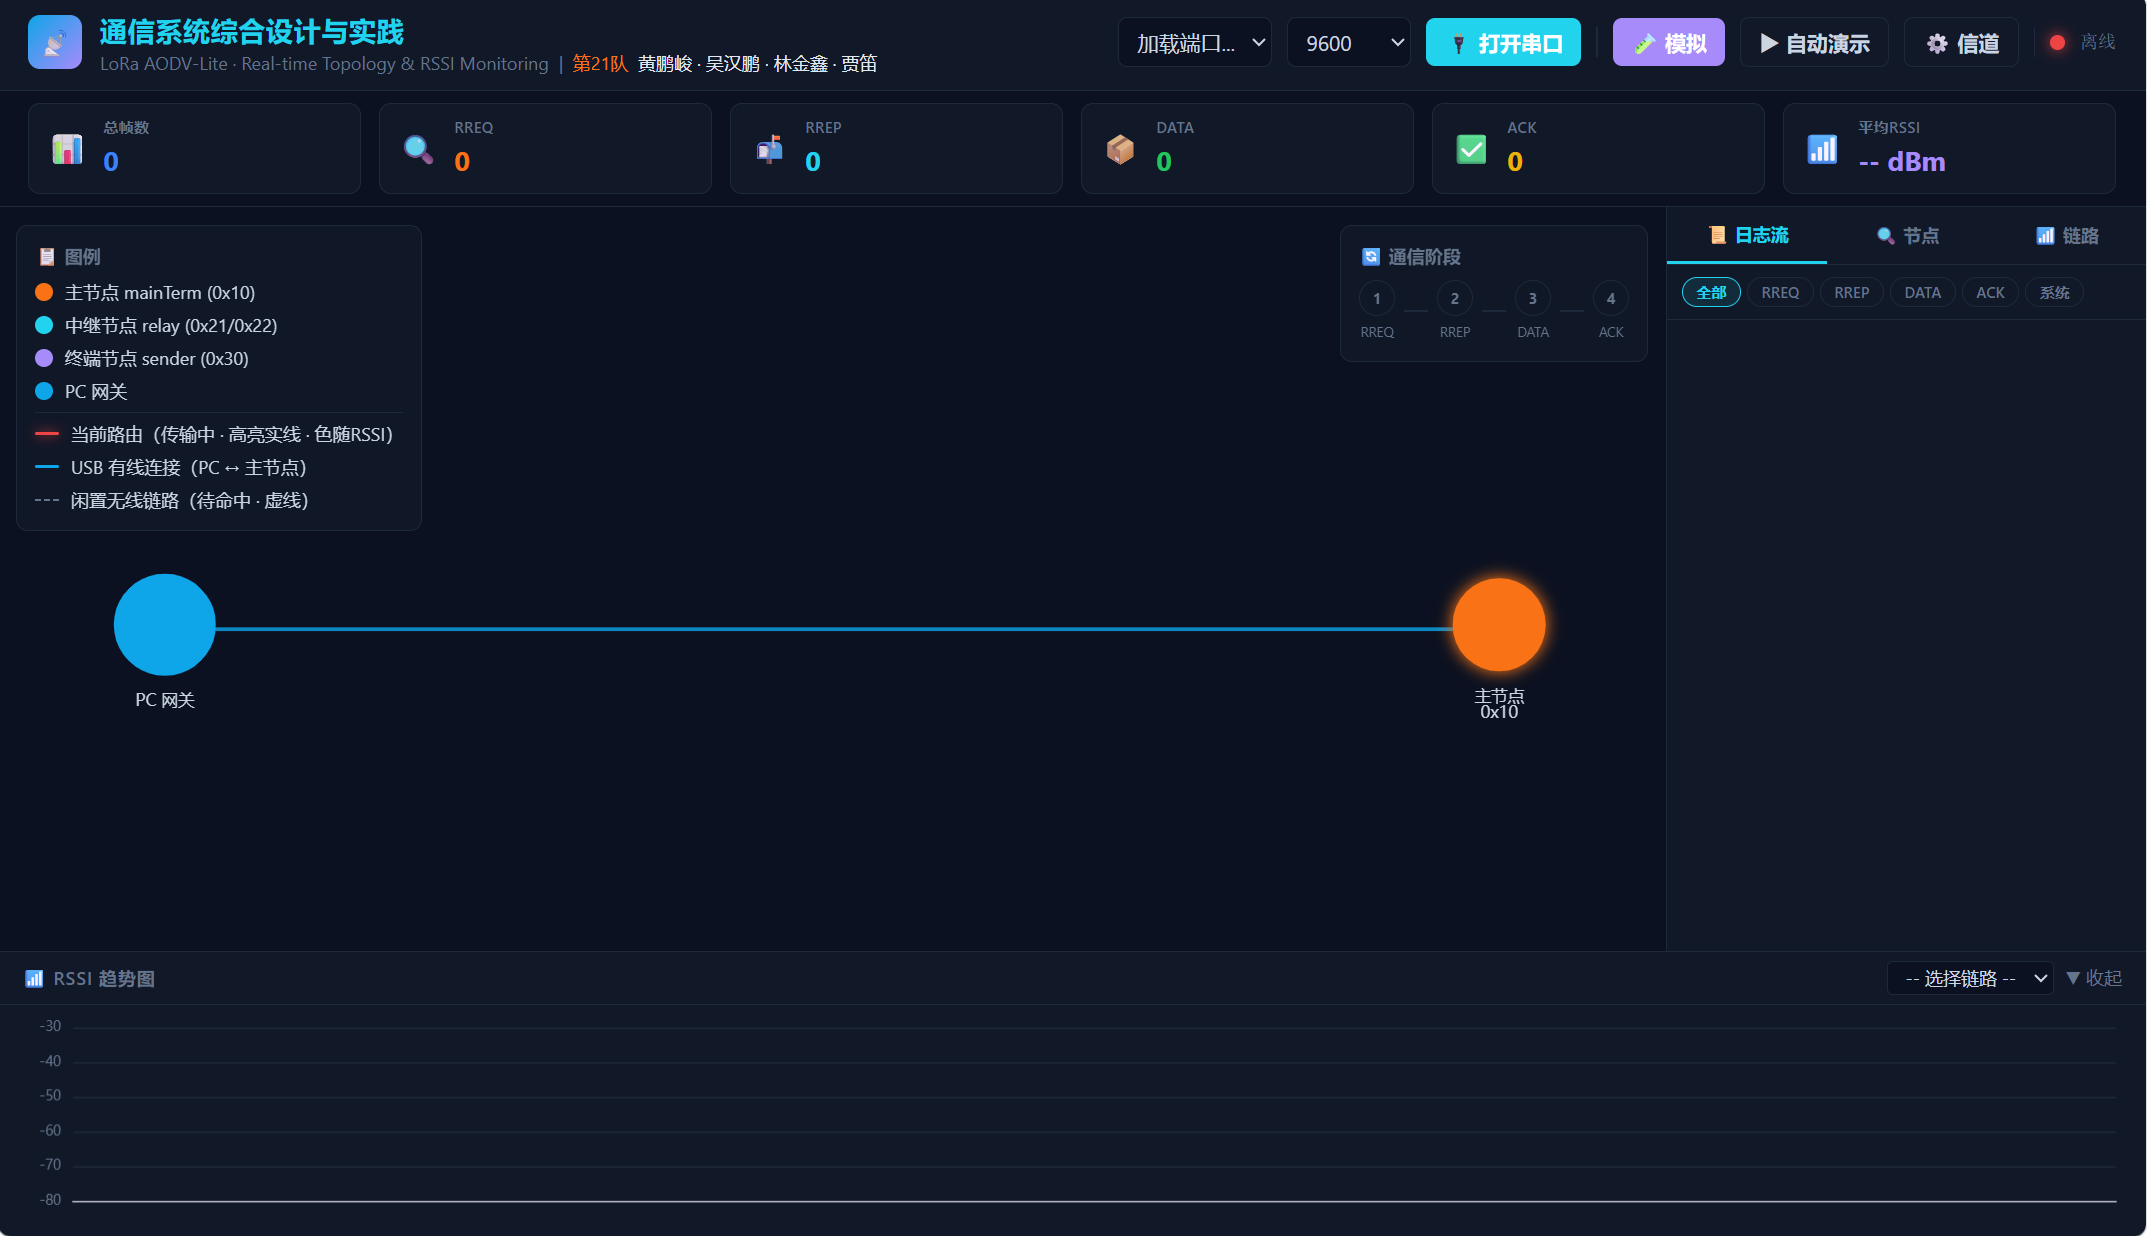
\includegraphics[width=\textwidth]{fig_ui_layout.jpg}
\caption{Web 前端页面布局}
\label{fig:uilayout}
\end{figure}

\begin{table}[htbp]
\centering
\caption{前端页面功能区}
\label{tab:frontendpanels}
\rowcolors{2}{tblrowA}{tblrowB}
\begin{tabularx}{\textwidth}{l >{\raggedright\arraybackslash}X}
\toprule
\rowcolor{tblhead}\tblheaderstyle 区域 & \tblheaderstyle 功能 \\
\midrule
Header 工具栏 &
项目标题、串口选择/波特率、打开/关闭串口按钮、模拟/自动演示/信道配置按钮、WebSocket 连接状态指示 \\

Stats Bar &
6 个统计卡片：总帧数、RREQ、RREP、DATA、ACK、平均 RSSI，数值颜色随数据动态变化 \\

拓扑图 &
ECharts 力导向图，节点坐标锁定以避免力模拟抖动，链路颜色按 RSSI 分级着色，当前路由高亮并带发光描边 \\

通信阶段指示器 &
4 步流程 RREQ $\to$ RREP $\to$ DATA $\to$ ACK，当前阶段放大高亮并附加脉冲动画，已完成步骤打勾标记 \\

图例 &
节点角色配色说明（橙=主节点、青=中继、紫=终端、蓝=PC）+ 链路线型释义（实线=传输中/USB、虚线=闲置） \\

日志流 Tab &
实时滚动日志，支持按消息类型（全部/RREQ/RREP/DATA/ACK/系统）一键过滤，每条日志展示源/目标/类型/pathId/印章/路径/data 原文 \\

节点详情 Tab &
点击拓扑图中任意节点自动跳转至此面板，列出 HEX ID、DEC ID、角色名称、最后活跃秒数、该节点关联的全部链路及实时 RSSI 值 \\

链路统计 Tab &
汇集所有活跃无线链路（USB 有线链路 PC-0x10 除外），标注 RSSI 数值、线型与宽度的物理含义、当前是否为传输路由 \\

RSSI 趋势图 &
底部可折叠折线图，以时间为 X 轴展示用户所选链路的最近 120 秒 RSSI 历史，支持从下拉框动态切换监控目标 \\

信道配置面板 &
右侧滑出式面板，选择目标节点、设置频率（MHz）/扩频因子（SF7--SF12）/发射功率（dBm），通过 WebSocket 经 mainTerm 下发至任意节点 \\
\bottomrule
\end{tabularx}
\end{table}

\paragraph{RSSI 颜色编码}
前端对信号强度采用五级颜色映射，每一级对应一个视觉直观的色彩和一个明确的 dBm 区间，如表~\ref{tab:rssicolor} 所示。这套配色方案直接取自 Tailwind CSS 的色板体系，确保了整体界面的视觉一致性。

\begin{table}[htbp]
\centering
\caption{RSSI 信号强度颜色映射}
\label{tab:rssicolor}
\rowcolors{2}{tblrowA}{tblrowB}
\begin{tabularx}{\textwidth}{c c c >{\raggedright\arraybackslash}X}
\toprule
\rowcolor{tblhead}\tblheaderstyle RSSI 范围 & \tblheaderstyle 颜色 & \tblheaderstyle 色码 & \tblheaderstyle 含义 \\
\midrule
$> -40$\,dBm           & 绿色  & \texttt{\#22c55e} & 信号优秀 \\
$-40 \sim -50$\,dBm    & 黄绿  & \texttt{\#84cc16} & 信号良好 \\
$-50 \sim -60$\,dBm    & 黄色  & \texttt{\#eab308} & 信号一般 \\
$-60 \sim -70$\,dBm    & 橙色  & \texttt{\#f97316} & 信号较弱 \\
$< -70$\,dBm           & 红色  & \texttt{\#ef4444} & 信号差 \\
未知                   & 灰色  & \texttt{\#6b7280} & 未收到 RSSI 数据 \\
\bottomrule
\end{tabularx}
\end{table}

\paragraph{拓扑节点垃圾回收}
前端以 4 秒为周期扫描全部活跃节点的时间戳。超过 20 秒未收到任何消息的非核心节点（PC 网关和 mainTerm 主节点被排除在回收范围之外，因为它们永远不会从网络中消失）将被自动从拓扑图中移除，其关联的所有链路一并清理。这一机制保证了前端拓扑图始终反映网络的当前真实状态，而非堆积历史幽灵节点。

\paragraph{自动演示模式}
在前端点击"自动演示"按钮后，系统以 6 秒为间隔循环触发 Python 后端的模拟通信接口，每轮包含完整的入网、心跳、RREQ 广播（含多路径印章）、RREP 选路、DATA 传输和 ACK 确认流程。RSSI 值在模拟中自动叠加随机漂移，使演示效果更接近真实无线信道的动态特性。

% ============================================================
\section{组网过程设计}
\label{sec:networking}
% ============================================================

\subsection{白名单入网机制}

\subsubsection{白名单策略}

系统采用硬编码于 mainTerm 固件的白名单作为入网安全的第一道门槛。白名单中预定义了所有合法节点的 ID 和角色，见表~\ref{tab:whitelist}。在当前的实验配置下，白名单包含 1 个主节点（自身）、2 个中继节点和 1 个终端节点。白名单扩展只需修改 mainTerm 固件中的对应数组并重新烧录，无需改动任何其他节点的代码。

\begin{table}[htbp]
\centering
\caption{系统白名单}
\label{tab:whitelist}
\rowcolors{2}{tblrowA}{tblrowB}
\begin{tabularx}{0.7\textwidth}{c c >{\raggedright\arraybackslash}X}
\toprule
\rowcolor{tblhead}\tblheaderstyle 节点 ID & \tblheaderstyle 角色 & \tblheaderstyle 说明 \\
\midrule
0x10 & 主节点   & 自身，无需入网 \\
0x21 & 中继节点 & 第一中继 \\
0x22 & 中继节点 & 第二中继 \\
0x30 & 终端节点 & 发送终端 \\
\bottomrule
\end{tabularx}
\end{table}

\subsubsection{入网流程（三次握手）}

节点上电后并不能立即参与网络通信，而是需要首先完成与主节点的三次握手入网过程。

第一步，新节点以 LoRa 广播方式发送 JOIN 帧（\texttt{msgType = 0x20}）。帧的 \texttt{data[0]} 字节写入本节点的角色码——1 表示中继节点，2 表示终端节点——目标地址固定为 \texttt{0x10}。

第二步，主节点收到 JOIN 请求后，提取发送者的 \texttt{srcId} 与本地白名单进行比对。若 \texttt{srcId} 在白名单中且角色码与预定义角色匹配，则回复 JOIN\_OK 帧（\texttt{msgType = 0x21}，\texttt{data[0..1] = 0xAC 0x00}），表示入网成功；若不匹配，则回复 JOIN\_NO 帧（\texttt{msgType = 0x22}）并在 \texttt{data[0]} 中携带拒绝原因码。

第三步，入网成功后的节点立即开始周期性发送心跳帧（\texttt{msgType = 0x03}），向主节点宣告自己的存活状态。心跳同时起到维持拓扑时效性的作用——若主节点超过 60 秒未收到某节点的心跳，则将其标记为离线。

\subsubsection{前端组网状态追踪}

前端 JavaScript 维护一个 \texttt{joinedNodeSet} 集合，每当收到 JOIN\_OK 帧时便将对应节点 ID 加入该集合。当三个远程节点（0x21、0x22、0x30）全部完成入网后，\texttt{networkReady} 标志被置为 true。在此之前，串口文本日志在前端不予显示——这是为了避免系统启动期间海量的初始化日志淹没用户真正关心的通信数据。这种延迟展示策略显著改善了前端日志面板的可读性。

\subsection{AODV-Lite 路由发现流程}

AODV-Lite 协议是本系统的核心路由算法，它在经典 AODV 协议的基础上做了两项关键简化：以单调递增的 pathId 取代复杂的序列号机制，以瓶颈 RSSI 比较取代跳数优先的路由度量。完整的通信流程可以分为四个界限分明的阶段。

\subsubsection{第一阶段：RREQ 路由发现}

当终端节点 sender 的路由缓存失效或过期时，它构造一个 \texttt{count = 0}、\texttt{pathId} 递增的 RREQ 帧并向空中广播。所有处于接收状态的中继节点收到该广播后，并不是简单地将帧原样转发，而是执行 RSSI 盖章操作——将本节点的 ID 和收到该帧时的 LoRa 信号强度（int8 格式）追加写入帧的 data 区，然后重新广播。

在多跳场景下，这一过程会形成一条完整的"数字足迹"：sender 的原始 RREQ 首先被第一跳中继（如 0x21）盖章并转发，随后被第二跳中继（如 0x22）再次盖章并转发。当这些携带了沿途各跳 RSSI 印章的 RREQ 副本最终到达 mainTerm 时，主节点便拥有了一份详细的"路径信号地图"——它能够看到每条候选路径上每一个中继节点的接收信号强度。

\subsubsection{第二阶段：路径裁决与 RREP}

mainTerm 在 500\,ms 的窗口内耐心收集同一 pathId 的所有 RREQ 副本——来自直达路径的、经 0x21 单跳的、经 0x22 单跳的、甚至经 0x21 再到 0x22 双跳的。窗口关闭后，mainTerm 首先对收集到的候选路径进行去重合并（同路径多副本仅保留瓶颈 RSSI 最好的版本），然后按瓶颈 RSSI 的取值分离出直达最优和中继最优。

裁决的原则在前文已经阐明：若中继路径的瓶颈 RSSI 大于或等于直达路径的瓶颈 RSSI，则选择中继；否则选择直达。裁决结果被写入一个 RREP 帧的 \texttt{data[]} 字段——这就是选中路径的中继 ID 列表——然后沿原路回传给 sender。

中继节点在收到 RREP 时执行选择性转发：检查本节点的 ID 是否出现在中继列表中，若出现则透明转发，若未出现则沉默。

\subsubsection{第三阶段：DATA 数据传输}

sender 收到 RREP 后，从中提取选中的中继 ID 列表，将其存入本地路由缓存，然后立即沿该路径发送 DATA 帧。DATA 帧的载荷部分由两个字节组成：一个单调递增的 sampleCounter 和一个固定的魔数 0xAB。路径上的每一个中继——只要本节点 ID 在 \texttt{data[]} 中继列表里——便有义务将 DATA 帧透明转发至下一跳，直到帧抵达 mainTerm。

\subsubsection{第四阶段：ACK 确认}

mainTerm 成功收到 DATA 后，不经过任何延迟便沿原路径回传 ACK 帧。为了最大化 ACK 到达 sender 的概率，mainTerm 连续发送 3 份 ACK（每份间隔 80\,ms），途经的中继节点则将这个冗余级数降为 2 份——这是一种依据重要性逐级递减的分级冗余策略。

sender 一旦收到任何一份 ACK，便确认本轮传输成功，随即强制清除路由缓存并进入 10\,s 的静默等待期。如果在 2\,s 内未收到任何 ACK，则标记路由为无效，等待静默期结束后重新发起 RREQ 探测。

\begin{figure}[htbp]
\centering
\includegraphics[width=0.75\textwidth]{fig_comm_sequence.jpg}
\caption{AODV-Lite 完整通信时序：RREQ 路由发现 $\to$ RREP 路径应答 $\to$ DATA 数据传输 $\to$ ACK 确认}
\label{fig:commseq}
\end{figure}

图~\ref{fig:commseq} 以时序图的视角将上述四个阶段压缩在一张图内。图中四根生命线分别代表 sender、relay(0x21)、relay(0x22) 和 mainTerm，不同颜色的箭头对应不同阶段：橙色代表 RREQ 广播与印章链，青色代表 RREP 沿选定路径回传，绿色代表 DATA 上行传输，黄色代表 ACK 分级下行确认。

\subsubsection{每轮重新探测的设计理由}

外行人可能会提出疑问：既然已经找到了一条好路径，为什么不在后续通信中持续复用？答案在于无线信道的时变特性。LoRa 信号在 530\,MHz 频段上的传播受多种因素影响——室内人员的走动导致多径模式改变、相邻频段的突发干扰、甚至天气湿度的变化都会微妙地影响信号衰减。上一轮表现优异的路径，数秒后可能因一个简单的物理遮挡而质量骤降。强制每轮重新探测，虽然在理论上增加了探测开销，但在实践中确保了当前使用的路径始终反映此刻的真实电磁环境。对于以可靠性为首要目标的系统而言，这是一个清醒的权衡。

\subsection{组网过程状态转移}

\subsubsection{节点侧状态转移}

从单个节点上电到正式融入网络，其生命周期经历的状态转移如图~\ref{fig:nodejoin} 所示。

\begin{figure}[htbp]
\centering
\includegraphics[width=0.88\textwidth]{fig_node_join_state.jpg}
\caption{节点入网状态转移图}
\label{fig:nodejoin}
\end{figure}

图~\ref{fig:nodejoin} 描述了一条完整的入网轨迹：上电后处于"未入网"孤立状态，随即广播 JOIN 请求并进入"等待应答"状态。如果收到主节点的 JOIN\_OK 帧，则切换为"已入网"在线状态，之后每 30 秒周期性发送心跳，同时参与到 AODV-Lite 路由发现的过程中。如果收到 JOIN\_NO 帧，说明白名单校验未通过，节点转入"被拒绝"状态并保持静默。如果在 3 秒内未收到任何应答，节点重发 JOIN 请求——最多尝试 3 次。此外，一旦主节点检测到已入网节点超过 60 秒未发送心跳，则将其标记为离线并从活跃拓扑中移除。

\subsubsection{网络侧状态转移}

从整个网络的宏观视角看待状态变化，则形成如图~\ref{fig:netstate} 所示的格局。

\begin{figure}[htbp]
\centering
\includegraphics[width=0.88\textwidth]{fig_network_state.jpg}
\caption{网络组网状态转移图}
\label{fig:netstate}
\end{figure}

图~\ref{fig:netstate} 区分了两个宏观状态：在"组网中"状态下，仅有部分节点完成了入网，网络尚未具备完整的通信能力；当所有节点全部完成 JOIN\_OK 且 \texttt{networkReady} 标志为 true 后，网络进入"网络就绪"状态，此时正常的 AODV-Lite 通信流程正式开始。在"网络就绪"状态下，系统同时面临三条并行路径：其一，sender 每 10 秒发起一轮正常通信，ACK 成功后清除路由并等待下一轮；其二，若某节点因断电或超出通信范围而离线（超过 60 秒无心跳），拓扑图自动更新并触发告警通知，网络退回到"组网中"状态等待该节点恢复；其三，若有新节点动态加入——例如实验中途额外上电第二台中继——系统通过 JOIN 协议接纳新节点，拓扑图扩展，网络在"网络就绪"状态下直接扩展规模。

\subsection{网络维护机制}

\subsubsection{心跳保活}

入网成功的节点不会沉默等待——它们以大约 30 秒为周期主动向主节点发送心跳帧，这个看似微小的动作维持了整个网络的"脉搏"。主节点据此记录每个节点的最后活跃时间戳。心跳机制在概念上类似于 TCP 的 keepalive，但在实现上极度轻量：一个 16 字节的帧，msgType 字段填入 0x03，仅此而已。

\subsubsection{拓扑超时清理}

系统在三个层面维护了拓扑的时效性。前端层面，JavaScript 定时器每 4 秒扫描活跃节点列表，超过 20 秒无消息更新的非核心节点被移除并生成一条 \texttt{[离线]} 日志。后端层面，Python StatsTracker 为每个节点维护 \texttt{lastSeen} 时间戳，可通过 API 接口查询。主节点层面（作为可扩展能力），若某节点超过 60 秒未发送心跳，则将其移出白名单活跃列表。

\subsubsection{路由老化}

除了主动的 ACK 后清除路由之外，sender 的路由缓存还设有一个被动的 10 秒有效期。即使因为某种原因 sender 始终未发起新通信，超过有效期的路由也会被自动标记为无效，下一轮自动触发 RREQ。这种双重保障（主动清除 + 被动老化）确保了路由信息不会在电磁环境已经变化的情况下被盲目信任。

\subsubsection{网络状态告警}

前端界面通过多条途径实时呈现网络的健康状况。WebSocket 连接指示灯以绿色或红色圆点直接反映数据通道的连通性；拓扑图中节点超时自动消失并伴随系统日志记录；Python 后端在串口异常时自动广播 \texttt{sys\_error} 类型的 WebSocket 消息；组网完成之前，串口的文本日志暂不显示——这看似是隐藏信息，实则是一种"有意义的沉默"，避免了启动阶段的海量噪音淹没真正的通信数据。

\subsubsection{网络参数在线调整}

系统具备在不中断运行的情况下在线调整任意节点信道参数的能力。操作路径清晰而完整：用户在浏览器右侧滑出的"信道配置"面板中选择目标节点（0x10、0x21、0x22 或 0x30），设置希望的频率值、扩频因子和发射功率，点击下发。前端将参数封装为 \texttt{CFG:<node>:F<freq>:S<sf>:P<power>} 格式的命令字符串，经 WebSocket 抵达 Python 后端，再通过串口写入 mainTerm。mainTerm 解析命令后，通过 LoRa 单播至目标节点。目标节点收到后立即执行参数调整，并通过串口打印确认信息。这一功能完整覆盖了课程提高要求中"任意节点的信道可读、可设置、可显示"的指标。

\subsection{动态节点加入}

系统对新节点的加入持欢迎态度。无论在网络组建初期还是正常运行期间，只要有新节点上电并发送 JOIN 请求，主节点就会执行白名单校验。校验通过后，新节点获得入网许可，前端自动将其添加到拓扑图中，并且从下一轮 RREQ 探测开始，新节点（如果是中继）就会被纳入 RSSI 盖章和路径选择的候选范围。整个过程无需重启任何设备或中断正在进行的通信，实现了真正意义上的"即插即用"。这一设计覆盖了课程提高要求中"动态新加入节点，以 4 个节点（2 级中继节点）完成可靠通信"的指标。

% ============================================================
\section{可靠通信设计}
\label{sec:reliability}
% ============================================================

\subsection{瓶颈 RSSI 选路算法}

在多跳无线网络中，路径选择的核心困难在于如何用一个单一的数值来评价一条由多段链路串联而成的路径的质量。常见的做法是计算路径的平均 RSSI——这种方法计算简单，但有一个致命的缺陷：平均值会掩盖最差的链路。设想一条路径上有三段链路，RSSI 分别为 $-70$\,dBm、$-40$\,dBm 和 $-40$\,dBm，平均值约为 $-50$\,dBm，看起来尚可接受。然而实际上，$-70$\,dBm 的那一段已经接近 LoRa 的接收灵敏度极限，该段链路的丢包率可能远高于另外两段，整条路径的可靠性本质上由这最差的一跳决定。

基于这一认识，本系统采用瓶颈 RSSI 策略：路径的质量 = $\min(\text{路径上所有跳的 RSSI})$。在候选路径中选择瓶颈 RSSI 最大的那条——换言之，选择"最不差"的路径。这背后的工程直觉是：与其追求某几跳信号特别强，不如确保没有任何一跳的信号特别弱。

\subsection{非阻塞中继转发}

传统的中继实现通常在收到 RREQ 后立即调用 LoRa 发送函数进行转发，发送期间 CPU 被阻塞在等待发送完成的循环中，无法接收任何新帧。这在多中继场景下会引发两个严重的问题。第一，如果两个中继几乎同时收到同一个广播 RREQ 并都在"立即转发"，它们的发送时机高度重叠，在空中发生碰撞的概率极大。第二，阻塞式 delay 导致的 RX 盲区会使中继错过后续中继的 RREQ 转发，从而在多跳场景（如 sender $\to$ relayA $\to$ relayB $\to$ mainTerm）中断裂转发链条——relayB 可能永远收不到 relayA 的转发帧。

本系统通过非阻塞队列设计解决了这两个问题。收到 RREQ 后并不立即发送，而是根据本节点的 ID 计算出差异化的退避时间（0x21 退避 90\,ms，0x22 退避 170\,ms），然后将盖章后的帧放入容量为 2 的 pending 队列。主循环中的 \texttt{servicePending()} 函数以异步方式逐个发送队列中的帧，两次发送之间间隔至少 30\,ms。这个时间窗口确保了中继在两次发送之间有足够的机会切换回收听模式。

\subsection{转发去重保护}

LoRa 网络的广播特性意味着同一个帧可能经过不同的路径被同一个中继多次收到。举例来说，中继 B 可能首先收到中继 A 对 sender RREQ 的转发，略晚一些又收到 sender 原始 RREQ 的直接广播——如果 B 不加以区分，会将同一个 RREQ 盖章并转发两次。在更复杂的拓扑中，多个中继之间的交叉覆盖甚至可能形成环路。

去重保护通过维护一个容量为 4 的环形缓存实现，每条记录为一个四元组 \texttt{(srcId, destId, pathId, msgType)}。每次准备转发前，线性扫描该缓存进行精确匹配。匹配成功意味着该四元组已被处理过，直接丢弃。在 RREQ 的特殊情况下，去重逻辑进一步细化——不仅检查四元组，还比较印章中的中继 ID 链是否完全相同，相同则只保留瓶颈 RSSI 更好的那个版本。

\subsection{ACK 分级冗余策略}

ACK 是整个传输过程的最后一步，也是最重要的确认信号。倘若 ACK 在回传途中丢失，sender 将误认为传输失败，不仅浪费了已经成功送达的数据，还会触发不必要的新一轮路由探测。为此，本系统设计了分级冗余策略，见表~\ref{tab:ackredundancy}。

\begin{table}[htbp]
\centering
\caption{ACK 分级冗余策略}
\label{tab:ackredundancy}
\rowcolors{2}{tblrowA}{tblrowB}
\begin{tabularx}{\textwidth}{l c >{\raggedright\arraybackslash}X}
\toprule
\rowcolor{tblhead}\tblheaderstyle 节点 & \tblheaderstyle ACK 副本数 & \tblheaderstyle 原因 \\
\midrule
mainTerm (源发) & 3 份，间隔 80\,ms & ACK 是关键确认，丢失将导致整轮传输失败，需最大冗余 \\
中继 (转发)    & 2 份，间隔 80\,ms & 降级冗余，平衡可靠性与信道占用 \\
sender (终点)  & --                & 不发送 ACK，只等待接收 \\
\bottomrule
\end{tabularx}
\end{table}

冗余递减的逻辑是：越靠近源头的节点，ACK 丢失的后果越严重（后续所有中继都无法转发），因此应该发送更多副本。中间节点只需保证有足够的机会将 ACK 送到下一跳即可，冗余可以适当降低。

\subsection{超时与重试策略}

表~\ref{tab:timeouts} 汇总了系统涉及的全部超时参数及其设置依据。每一个参数的选择都经过了权衡：取得太短会导致不必要的超时和误判，取得太长会延缓系统对故障的反应速度。

\begin{table}[htbp]
\centering
\caption{系统超时参数汇总}
\label{tab:timeouts}
\rowcolors{2}{tblrowA}{tblrowB}
\begin{tabularx}{\textwidth}{l c >{\raggedright\arraybackslash}X}
\toprule
\rowcolor{tblhead}\tblheaderstyle 参数 & \tblheaderstyle 值 & \tblheaderstyle 说明 \\
\midrule
RREQ 收集窗口  & 500\,ms    & mainTerm 收集同 pathId 的 RREQ 的最大等待时间 \\
RREP 超时     & 2000\,ms   & sender 等待 RREP 的最长时间 \\
ACK 超时      & 2000\,ms   & sender 等待 ACK 的最长时间 \\
路由有效期     & 10000\,ms  & sender 路由缓存的最大年龄 \\
拓扑超时       & 20000\,ms  & 前端节点无消息更新的移除阈值 \\
心跳间隔       & $\sim$30\,s& 各节点向 mainTerm 发送心跳的周期 \\
通信间隔       & 10000\,ms  & sender 发起下一轮传输的静默等待时间 \\
\bottomrule
\end{tabularx}
\end{table}

值得特别说明的是 RREQ 收集窗口的 500\,ms 设置。对于 ATmega328P 主控的 LoRa 节点而言，SF7 下的单帧空中时间约为 50\,ms，加上中继的退避和转发延迟，一个经过双跳中继的 RREQ 副本从 sender 发出到抵达 mainTerm 大约需要 200 至 400\,ms。500\,ms 的窗口在确保收集到所有可能路径的 RREQ 的同时，也足够短以至于不影响用户体验。

% ============================================================
\section{软件模块设计}
\label{sec:modules}
% ============================================================

\subsection{系统软件模块划分}

系统软件按照功能归属和运行平台自然地分为三个层次，每个层次内部包含若干独立但协作的模块。

无线节点层运行在 Arduino 硬件上，包含三个固件模块。模块 A 是 sender 固件，其核心是一套三状态有限状态机，负责路由发现发起和数据发送。模块 B 是 relayTerm 固件，以非阻塞队列和退避算法为核心竞争力，实现 RREQ 的智能转发。模块 C 是 mainTerm 固件，兼具路由裁决者和串口桥接器两种身份。

PC 服务层运行在 Python 环境中，包含两个模块。模块 D 是串口解析引擎，它将 stats 追踪、二进制帧解析和文本行过滤封装在一个 StatsTracker 类和一个独立的读取线程中。模块 E 是 WebSocket 服务，基于 ConnectionManager 管理所有浏览器连接并以广播方式推送实时数据。

PC 表示层位于浏览器端，仅包含一个模块 F——Web 可视化前端。它不依赖任何前端框架，以原生 JavaScript 驱动 ECharts 图表和 WebSocket 通信。

\begin{figure}[htbp]
\centering
\includegraphics[width=0.9\textwidth]{fig_software_modules.jpg}
\caption{系统软件模块层次架构}
\label{fig:modules}
\end{figure}

图~\ref{fig:modules} 将这三层六模块的组织关系以层次图的形式直观呈现出来，层与层之间的数据流向也在图中一并标注。

\subsection{模块间接口}

上述六个模块之间通过六条明确定义的接口实现数据交换。接口的物理介质、协议格式和承载内容各不相同，但每一条接口的边界都十分清晰——这正是模块化设计的精髓所在，见表~\ref{tab:interfaces}。

\begin{table}[htbp]
\centering
\caption{模块间接口定义}
\label{tab:interfaces}
\rowcolors{2}{tblrowA}{tblrowB}
\begin{tabularx}{\textwidth}{c l l >{\raggedright\arraybackslash}X}
\toprule
\rowcolor{tblhead}\tblheaderstyle 接口 & \tblheaderstyle 方向 & \tblheaderstyle 协议/格式 & \tblheaderstyle 说明 \\
\midrule
I1 & sender $\leftrightarrow$ relay   & LoRa 530MHz          & 16B 帧，SF7，RSSI 盖章 \\
I2 & relay $\leftrightarrow$ relay    & LoRa 530MHz          & 16B 帧，透明转发 \\
I3 & relay $\leftrightarrow$ mainTerm & LoRa 530MHz          & 16B 帧，含末跳 RSSI \\
I4 & mainTerm $\to$ Python            & USB Serial 9600      & 16B 二进制帧 + ASCII 文本行 \\
I5 & Python $\to$ mainTerm            & USB Serial 9600      & ASCII 命令 \\
I6 & Python $\leftrightarrow$ Browser & WebSocket            & JSON \\
\bottomrule
\end{tabularx}
\end{table}

\begin{figure}[htbp]
\centering
\includegraphics[width=\textwidth]{fig_module_interfaces.jpg}
\caption{系统模块间接口示意}
\label{fig:interfaces}
\end{figure}

图~\ref{fig:interfaces} 将表~\ref{tab:interfaces} 定义的六条接口映射到实际的系统组件连接关系上。I1 至 I3 属于无线接口，它们共享相同的 LoRa 物理层但在应用层存在差异——I1 携带 RSSI 印章，I2 执行透明转发，I3 额外包含末跳 RSSI 信息。I4 和 I5 共享同一根 USB 线缆，但方向相反、功能各异：I4 上行传输 16 字节二进制帧和 ASCII 文本行，I5 下行传输命令字符串。I6 是唯一一条全双工双向通道，以 JSON 为载体在 Python 和浏览器之间交换结构化数据。

% ============================================================
\section{组网设计方案综合}
\label{sec:comprehensive}
% ============================================================

\subsection{入网方案}

如第~\ref{sec:networking} 节所述，入网采用白名单加三次握手的组合策略。新节点上电后广播 JOIN 帧，主节点依据硬编码白名单做出允许或拒绝的裁决，入网成功的节点进入周期性心跳维持的在线状态。这套流程简洁而完整——没有复杂的密钥交换，没有证书链验证，但在实验网络的规模和威胁模型下，已经提供了足够的安全保障。

\subsection{网络维护方案}

网络维护是一个持续的过程，而非一次性动作。心跳机制让主节点始终掌握全网节点的存活脉搏；前端的 20 秒超时扫描和后端的 StatsTracker 时间戳记录构成了两层拓扑时效性保障；sender 端的 10 秒路由老化和 ACK 后的主动清除路由形成了双重路由保鲜机制；中继的四元组去重缓存和主节点的窗口去重合并则在两个层面防止了冗余帧对网络资源的浪费。

\subsection{网络状态信息显示与告警方案}

前端界面充当了系统的"仪表盘"角色。ECharts 拓扑图以节点位置锁定、链路 RSSI 颜色编码和当前路由发光线三层叠加的方式，将网络的物理拓扑和逻辑路由同时呈现。四步通信阶段指示器（RREQ $\to$ RREP $\to$ DATA $\to$ ACK）则以动画形式让用户肉眼观察到通信流程的实时推进。六个统计卡片以秒级频率刷新帧计数和信号强度数据。实时日志流支持按消息类型一键过滤，将关键帧从信息洪流中提取出来。节点离线时，拓扑图自动移除对应节点并生成系统告警日志，用户无需主动检查即可感知网络变化。

\subsection{网络参数在线调整方案}

信道参数的调整范围覆盖了频率、扩频因子和发射功率三个最关键的射频参数。调整目标可以是网络中的任意节点，下发的指令沿 Browser $\to$ WebSocket $\to$ Python $\to$ Serial $\to$ mainTerm $\to$ LoRa $\to$ 目标节点的路径穿越整个系统栈。最关键的一点是，调整操作与正常通信可以并行进行——不需要暂停路由发现，不需要让节点离线，不需要重启任何设备。这种"在线可调"的能力使得系统在面对变化的电磁环境时具备了动态适应的灵活性。

\subsection{状态转换图汇总}

系统共涉及四个核心状态机，其状态转换图已在前文以图形方式呈现。sender 通信状态机（图~\ref{fig:senderfsm}）描述了终端节点在 IDLE、WAITING\_RREP 和 WAITING\_ACK 三个状态之间的循环切换。节点入网状态机（图~\ref{fig:nodejoin}）追踪了从孤立、等待、入网到可能离线的完整生命周期。网络组网状态机（图~\ref{fig:netstate}）则从整网视角划分了"组网中"和"网络就绪"两个宏观状态以及它们之间的转移条件。此外，mainTerm 的裁决过程本身也隐含着一个窗口状态机：空闲 $\to$ 收集 $\to$ 裁决 $\to$ 发送 $\to$ 回到空闲。

\subsection{伪代码设计汇总}

系统各核心模块的伪代码已在第~\ref{sec:nodes} 节中分别给出。sender 部分展示了主循环中对三个状态的判别与转移逻辑；relayTerm 部分涵盖了收包校验、RREQ 盖章入队和 RREP/DATA/ACK 选择性转发的完整函数链；mainTerm 部分则从最高层的 loop() 一直细化到 handleRREQ、evaluateAndReply、sendRREP 和 sendACK 等关键函数的内部逻辑。

% ============================================================
\section{扩展发挥}
\label{sec:extension}
% ============================================================

\subsection{实际应用场景}

本系统的技术方案并非仅限于实验室演示，它已经具备了向实用环境迁移的基本条件。

在环境监测领域，可以将温湿度、土壤墒情、空气质量等传感器集成到各 LoRa 节点上，利用多跳中继将分散在农田、森林或工业园区各处的传感数据汇聚至网关。PC 端不仅能够实时显示，还可以将历史数据存入本地数据库以供趋势分析。

在灾害应急通信场景下，当蜂窝网络因地震、洪水或台风而全面瘫痪时，救援队伍可以快速部署便携式 LoRa 中继节点，在数十分钟内构建起覆盖灾区的临时通信网络。虽然带宽有限，但足以传递求救信号、GPS 坐标和简短的文字信息——这些恰好是生死攸关时刻最需要传递的内容。

在智能楼宇监控应用中，多层建筑的本质就是一个天然的多跳拓扑——每层楼部署至少一个中继节点，地下室的水表和顶层的烟感报警器经由中间楼层的节点接力，最终将数据送达管理室的网关。相比于在整栋楼铺设有线传感器网络，LoRa 无线方案在施工成本和部署灵活性上具有显著优势。

\subsection{系统可扩展方向}

本系统在设计之初就为后续扩展预留了足够的空间。动态功率控制是一个自然的方向——根据实时 RSSI 反馈自适应调节发射功率，信号好时降低功率以节省电池，信号差时提高功率以确保连通。自适应数据速率同样是 LoRa 生态中的成熟技术，根据信噪比在 SF7 至 SF12 之间动态切换，能够在通信距离和数据速率之间找到最佳平衡。

在系统架构层面，部署多个主节点配合多个 PC 网关可以消除单点故障，这在需要高可用性的实际部署中是必不可少的。数据持久化方面，将 StatsTracker 的统计数据和 RSSI 历史存入 SQLite 或时序数据库，配合 Grafana 等可视化工具，可以构建出专业级的网络监控仪表盘。最后，通过 MQTT 协议将汇聚数据上传至云平台，可以实现真正意义上的远程监控——用户坐在家里的电脑前就能观察到几十公里外农田中的传感器读数。

% ============================================================
\section{团队分工设计}
\label{sec:team}
% ============================================================

\newpage

\begin{table}[H]
\centering
\caption{团队分工与贡献占比}
\rowcolors{2}{tblrowA}{tblrowB}
\begin{tabularx}{\textwidth}{c >{\raggedright\arraybackslash}X c}
\toprule
\rowcolor{tblhead}\tblheaderstyle 成员 & \tblheaderstyle 负责内容 & \tblheaderstyle 贡献占比 \\
\midrule
黄鹏峻 & Python 后端开发（FastAPI + WebSocket + 串口解析）、系统集成测试 & 25\% \\
吴汉鹏 & Web 前端开发（ECharts 拓扑 + 日志/节点/链路面板 + RSSI 趋势）、项目文档 & 25\% \\
林金鑫 & 终端节点固件（sender.ino）、中继节点固件（relayTerm.ino） & 25\% \\
贾笛   & 主节点固件（mainTerm.ino）、通信协议设计 & 25\% \\
\bottomrule
\end{tabularx}
\end{table}

以上分工反映的是每位成员的主要负责方向。在实际开发过程中，团队四人在各模块之间保持着密切的沟通与协作——固件开发者需要理解前后端接口的数据格式，前端开发者需要了解帧结构中各个字段的物理含义，后端开发者则需要掌握串口通信的时序特性。正是这种跨越分工边界的相互理解，使得整个系统的各个模块能够在联调阶段顺利地拼接为一个有机的整体。每位成员均深度参与了代码编写工作，满足课程对"每位同学完成相应设计工作（必须含程序编写）"的明确要求。

\end{document}
